\chapter{A Novel Spatial Feature for the Identification of Motor Tasks Using High-Density Electromyography}
\label{ch:4}
\textbf{Published as:} 
Jordanić, M., Roja-Martínez,  Ma\~nanas, M.A., Alonso J.F., Marateb H.R.
A Novel Spatial Feature for the Identification of Motor Tasks Using High-Density Electromyography 
\textit{Sensors} 17(7):1597, 2017

doi: 10.3390/s17071597

Impact Factor: 2.077; Position: 10 of 58 (Q1) INSTRUMENTS AND INSTRUMENTATION.


\textbf{Abstract:} Estimation of neuromuscular intention using electromyography (EMG) and pattern recognition is still an open problem. One of the reasons is that the pattern-recognition approach is greatly influenced by temporal changes in electromyograms caused by the variations in the conductivity of the skin and/or electrodes, or physiological changes such as muscle fatigue. This paper proposes novel features for task identification extracted from the high-density electromyographic signal (HD-EMG) by applying the mean shift channel selection algorithm evaluated using a simple and fast classifier-linear discriminant analysis. HD-EMG was recorded from eight subjects during four upper-limb isometric motor tasks (flexion/extension, supination/pronation of the forearm) at three different levels of effort. Task and effort level identification showed very high classification rates in all cases. This new feature performed remarkably well particularly in the identification at very low effort levels. This could be a step towards the natural control in everyday applications where a subject could use low levels of effort to achieve motor tasks. Furthermore, it ensures reliable identification even in the presence of myoelectric fatigue and showed robustness to temporal changes in EMG, which could make it suitable in long-term applications.

\textbf{Keywords:}  high-density electromyography; pattern recognition; myoelectric control; mean shift; prosthetics

\section{Introduction}

Electromyography (EMG) is a technique for recording the electrical activity produced by skeletal muscles. The EMG signal is a summation of action potentials produced by muscle fibers, directly triggered by the action potentials traveling along motor neurons [1]. Since EMG is an important source of neural information, it has been extensively studied in the field of human-machine interfacing [2,3]. Applications of EMG include the control of neurorehabilitation devices such as prostheses [4,5], rehabilitation robots [6,7], and identification of muscle anatomical structure [8], but also implementations in leisure activities such as sports [9] and computer games [10].

EMG signals could be recorded either non-invasively (surface EMG, sEMG) or invasively with needle and wire electrodes (intramuscular EMG, iEMG) [11]. Although the iEMG has higher signal-to-noise ratio, both approaches provide a similar quality of identification of upper-arm motor task [12]. Moreover, sEMG is preferred as it is recorded non-invasively.

The pattern recognition approach has been recently used in research laboratories as a state-of-the-art method to decode neural information. Its main advantage over conventional systems is the instant activation of a task belonging to any of the available degrees-of-freedom (DoFs). Many classifiers such as linear discriminant analysis (LDA), support vector machine, and artificial neural network were successfully employed for this purpose with a high identification fidelity [13], but many authors agree that the choice of the features is more important than the choice of the classifier [12]. Hence, simple and fast classifiers are preferred, among which the LDA is commonly used and has become a general recommendation [3,14]. In addition, different studies have focused on pattern recognition from the analysis of isometric contractions for myoelectric control, especially when considering subjects with neuromuscular impairment (in stroke for example) [15] and even for prostheses control for amputees [16]. Additional examples can be found in [17,18,19].

Features can be calculated in time, frequency/scale, and time-frequency/scale domain [2,3,13]. Time domain features are usually used because of their computational simplicity and good performance [3]. Additionally, they can be combined with other features to increase the performance, e.g., autoregressive features [12].

The influence of the physiological (e.g., muscle fatigue) or non-physiological (electrode-skin impedance) non-stationarity of the EMG features is a big issue in neuromuscular control. As a solution, Vidovic et al. [20] and Hahne et al. [21] proposed a real-time retraining of the classifier where the parameters are constantly updated. Liu et al. [22] proposed a universal LDA classifier which was trained during different days and then combined. Such methods adapt the model to changes in the features, rather than using robust features.
Moreover, the variation of force can affect the identification [23]. Scheme and Englehart [24] recommended to train the classifier using all effort levels, whereas He et al. [25] tackled the problem using a feature set based on the frequency content of the signal and muscle coordination.

With the recent introduction of high-density EMG (HD-EMG) [26], i.e., multichannel EMG recorded using 2D grids of closely spaced sEMG electrodes, multiple studies have reported improvement in task identification. Stango et al. reported that spatial features extracted from the HD-EMG are robust to the electrodes shift. Geng et al. [27] and Du et al. [28] exploited the power of deep convolutional network to design gesture recognition classifier that classifies instantaneous maps, i.e., raw HD-EMG samples. Hahne et al. extracted features using spatial filters optimized to increase separability between different classes [29]. This methods exploit the information about spatial muscle activation pattern extracted from the HD-EMG and the fact that the myoelectric activity over different parts of muscle depends on the various factors (e.g., contraction level [30], duration of the contraction [31], and joint position [32]) and can be useful in differentiation between tasks.

In our previous work, we used the center of gravity as a feature to describe spatial patterns in HD-EMG [18,19,33]. In this work, we propose a new spatial feature for task identification based on the modified mean shift algorithm. Novel features were evaluated in the identification of four isometric motor tasks of the upper-limb (flexion/extension, supination/pronation of the forearm) using the LDA classifier. The proposed features were tested in three conditions: when training set and test set were recorded at the same time (time-dependent changes in the signal are minor), when test set was recorded after training set, and during the fatiguing exercise. In addition, features were tested during the identification of task recorded at different effort levels. The proposed features proved to improve the identification and are especially useful in extreme cases like identification of tasks recorded at very low effort level or identification of tasks during fatigue. These results confirm the usefulness of information of spatial distribution of myoelectric intensity over the muscle in discrimination between tasks.
The rest of the paper is organized as follows: in the next section, information about the experimental protocol and the task identification method used in this study is presented. Section 3 provides the results of the identification using the proposed features and its comparison with the previously established features. The discussion is provided in Section 4 and finally, the conclusions are summarized in Section 5.\\
\clearpage

\section{Materials and Methods}

\subsection*{Instrumentation and Measurement Protocol}

Eight healthy subjects (age: 36 $\pm$ 5 years; height: 177 $\pm$ 5 cm; weight: 75 $\pm$ 9 kg; body mass index: 23.7 $\pm$ 2.3) participated in the experiment. They reported no pain, and previously had not suffered any injuries or neuromuscular upper limb impairments. The study was conducted in accordance with the Declaration of Helsinki and subsequent amendments concerning research in humans and was approved by the University Ethics Committee and the local government. Recordings and results were documented with the registration number, which corresponded to the Spanish ministry project MICINN (TEC2008-02274): “Analysis of the dynamic interactions in non-invasive multichannel biosignals for rehabilitation and therapy”. All subjects gave their written informed consent to participate in the experimental protocol.

Subjects performed four different isometric upper-limb tasks with two degrees of freedom: flexion/extension and supination/pronation of the forearm. During the experiment they were seated upright with their back being straight. Their dominant arm was positioned in the sagittal plane with the elbow flexed at 45 degrees and the forearm positioned in the middle between supination and pronation, thumb pointing upwards (Figure 1). To avoid muscle activation due to gripping, their hands were fixed at the wrist using a mechanical brace. The brace also contained two torque meters that measured exerted torque at the elbow joint.

HD-EMG was measured on five superficial muscles involved in the presented tasks: biceps brachii, triceps brachii, brachioradialis, anconeus, and pronator teres. Signals were recorded using three two-dimensional electrode arrays manufactured as silver-plated eyelets (2.5 mm radius) positioned in a quadrature grid with a 10 mm inter-electrode distance and embedded in a non-conductive fabric (Figure 1a).

After the skin was shaved, cleaned, and treated with abrasive gel, the following electrode arrays were positioned over the upper limb using elastic straps: two electrode arrays (dimensions: 8 rows × 15 columns) were positioned on the upper arm covering biceps brachii and triceps brachii muscles. The center of each electrode array was placed according to the positions recommended by the SENIAM project [34]. The third electrode array was placed over the forearm, with the first row of electrodes approximately 2 cm below elbow crest, covering brachioradialis, anconeus, and pronator teres muscles. A line connecting the origin and insertion of the targeted muscles were previously marked on the skin and the electrode array was placed to optimally cover these muscles. The forearm electrode array had six rows and between 17 and 19 columns, depending on the forearm circumference. After positioning the electrodes, the conductive gel was applied through the eyelet of each electrode (20 µL) using the dosimeter (Multipette Plus, Eppendorf, Germany).

HD-EMG signals were recorded in monopolar mode using three commercially available amplifiers with simultaneous sampling (EMG-USB, 128 channels, 2048 Hz sampling frequency, 10–750 Hz passband, manufacturer LISiN-OT Bioelettronica, Turin, Italy). Torque exerted on the elbow joint was measured using two torque transducers (OT Bioelettronica, range 150 Nm) and was displayed to the patient in real time. The detailed information on the instrumentation settings can be found in [35].

Prior to the experiment, the maximal voluntary contraction (MVC) was measured for each task as the maximal of three consecutive trials. In the first part of the experiment subjects were instructed to perform four defined tasks at three randomized different effort levels: 10\% MVC, 30\% MVC, and 50\% MVC. Having been instructed to maintain the target level for 10 s, the exerted torque was displayed to the subjects. Tasks were performed in random order and between two consecutive recordings there was a two-minute rest to prevent cumulative fatigue.

Approximately 30 min (33 $\pm$ 3 min) after the first part of the protocol, endurance measurements were performed. Subjects were instructed to perform each task at 50% MVC until failure. After each measurement, subjects rested for five min.

\subsection{Simulated data}

In order to simulate real cases of MEG signals affected by metallic interference, a linear mixture between clean signals and metallic artifacts extracted from contaminated signals was proposed, following a scheme analogous to that proposed in \citep{Romero2008} for the generation of simulated signals affected by ocular artifacts. Ten two-minute epochs were simulated according to the following mixing model:

\begin{equation} \label{eq:1-1} 
S=C+WP
\end{equation}

where $S$ indicates the simulated signals, $C$ denotes clean MEG recordings, $W$ corresponds to the mixture weights, and $P$ represents the different artifactual morphologies selected. These different patterns caused by metallic interference had to be extracted from contaminated recordings and then added to clean signals according to the propagation coefficients obtained by means of an approach based on linear regression.

\subsubsection*{Extraction of different metallic artifactual waveforms from contaminated recordings}

Most noticeable metallic artifacts are easily identifiable on visual inspection of the signals mainly due to their higher amplitude with respect to the remaining MEG channels, but also to their slower and more regular waveforms, which are usually modulated by the heart or respiratory rates \citep{Hillebrand2013}. In this study, three experts examined the signals and identified channels that clearly and strictly met these criteria of high amplitude, low frequency, regularity, and possible modulation by respiratory or cardiac rhythms. Only those channels selected by all three experts were chosen as artifactual channels and therefore used to obtain the artifactual waveforms. The interobserver agreement was of 0.829 $\pm$ 0.097 with a kappa index of 0.851 $\pm$ 0.095, indicating an 'almost perfect' agreement according to the definitions given in \citep{Viera2005}.

In order to extract only the information provided by metallic interference, a low-pass filter with the cutoff frequencies obtained with the cumulative spectra was applied to remove the cerebral activity present in these selected channels (7.4 $\pm$ 2.1 Hz as mean and standard deviation for all channels). The spectra of clean and artifactual signals were similar at high frequencies but they differed at low frequencies due to metallic interference. Considering that this conspicuous difference was due to the presence of the metallic artifact, reverse-cumulative (from high to low frequency) spectra were obtained for each artifactual channel and for the same channel in all artifact-free recordings. Spectra were calculated by means of Welch's periodogram using a five-second Hanning window with 50\% overlapping. The difference between the artifactual spectrum and the average of all clean spectra was used to obtain the cutoff frequency for each artifactual channel, searching for the frequency where the normalized difference reached 5\% (see figures \ref{fig:1-1}(a) and (b)). Subsequently, each selected artifactual channel was filtered with an 8th-order Butterworth filter (figure \ref{fig:1-1}(b)).

\begin{figure}[ht]
\centering
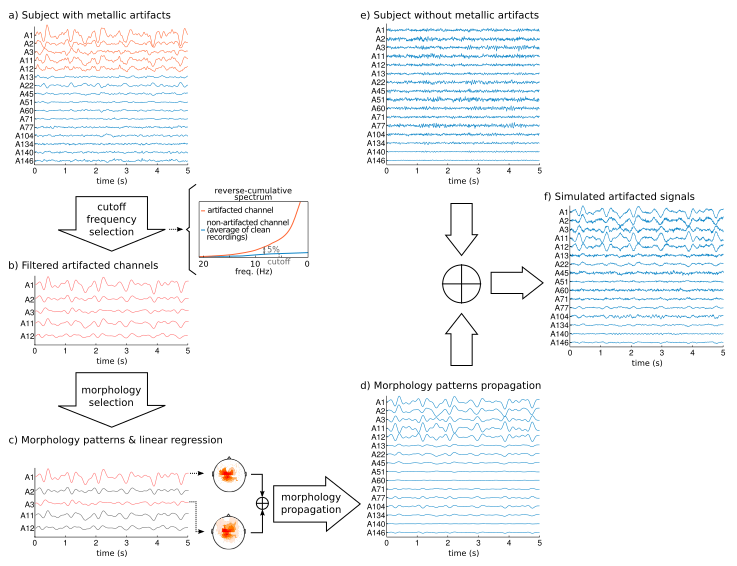
\includegraphics[width=1\textwidth]{Images/fig1-1.png}
\caption{Scheme for generation of a simulated artifactual MEG recording: (a) five-second epoch of raw MEG with metallic artifacts (only 16 selected channels are drawn). Orange traces correspond to the highly artifactual channels selected by the experts; (b) low-pass filtered artifactual channels (cutoff frequency automatically calculated from reverse-cumulative spectra); (c) selected morphologies (orange traces) after correlation among channels in (b), and their corresponding linear regression coefficients (whole head maps); (d) propagation of artifacts corresponding to coefficients obtained in (c); (e) five-second epochs of raw artifact-free MEG channels; and (f) simulated signals obtained by summation of (d) and (e).}
\label{fig:1-1}
\end{figure}      

Metallic interference is known to affect different MEG channels with varying shape and intensity. For this purpose, a selection of the different waveforms spreading over the scalp had to be performed. Consequently, the cross-correlation between artifactual channels was obtained, and only low-correlated waveforms (coefficient $<$ 0.5) were preserved. Among those showing high correlation ($\geq$ 0.5), only the signal with the highest energy was maintained (see figure \ref{fig:1-1}(c)). In this way, only those morphologies that were different enough were selected as artifactual patterns (figure \ref{fig:1-1}(d)).

\subsubsection*{Calculation of propagation coefficients by linear regression and generation of simulated data}

Propagation coefficients represented the amount of metallic interference that was present in a particular MEG channel with respect to a specific artifactual pattern. Linear regression between all channels of the actual artifactual recordings and each selected pattern was performed, taking into account the entire two-minute recordings. The obtained regression coefficients (represented as topographic maps in figure \ref{fig:1-1} (c)) were used as weights of the mixing matrix \textbf{\textit{W}} (equation \ref{eq:1-1}) and then patterns were propagated to all channels (figure \ref{fig:1-1}(d)). Finally, the simulated artifacts were added to clean recordings (figure \ref{fig:1-1}(e)) to obtain a set of simulated artifactual signals (figure \ref{fig:1-1}(f)). These steps were performed 10 times to obtain 10 sets of simulated MEG signals with known metallic interference.

\subsection{Blind source separation approaches to artifact reduction}

BSS techniques estimate source signals from a set of mixed signals, separating MEG signals into spatial components to later reconstruct the brain signal discarding the components associated with artifacts. The model of the identification process is expressed by:

\begin{equation} \label{eq:1-2}
x(t)=As(t)
\end{equation}

where $x(t)$ is the observation signal vector and $s(t)$ the unknown source signal vector with \textit{n} and \textit{m} rows respectively. $A$ is the $n \times m$ mixing matrix which should be estimated and represents the weights of the projection of the corresponding source signals at different channels.

Usually, BSS methods can be classified according to the order of the statistic used to perform the separation. Methods based on second order statistics (SOS) assume sources that are only uncorrelated. One of the techniques used in this study is the Algorithm for Multiple Unknown Signals Extraction (AMUSE) \citep{Tong1991}, which exploits SOS through a first step of signal whitening and a second step of an eigenvalue decomposition. AMUSE is sometimes classified as an independent component analysis (ICA) technique because decorrelation can be considered as a weak form of statistical independence \citep{Hyvarinen2001}. However, SOS are effectively enough to separate and remove those Independent Components (IC) corresponding to various types of artifacts \citep{Escudero2010}.

While SOS-based algorithms provide independence in terms of correlation, in the case of higher order statistics (HOS) a more general concept in considered: two random variables are independent when the statistical behavior of one of them is not affected by the values taken by the other. Statistical independence can be estimated using several different methods based on mutual information, non-gaussianity or maximum likelihood, for example. Additionally to AMUSE, two HOS-based techniques, INFOMAX and FastICA, were used in this work. Both algorithms are iterative and require proper initialization and parameter setting.

On the one hand, INFOMAX maximizes the joint entropy of a neural processor output, based on the fact that the maximum entropy of joint variables only occurs when they are statistically independent \citep{Bell1995}. In this study, separation by means of an extended version of INFOMAX was performed using the default parameters proposed in the EEGLAB toolbox for MATLAB \citep{Delorme2004,Lee1999}

On the other hand, FastICA is based on a fixed-point iterative scheme that maximizes non-gaussianity as a measure of statistical independence between sources. A weight matrix is obtained after a certain number of iterations, but non-gaussianity of the independent components is necessary for a successful convergence of the algorithm \citep{Hyvarinen1999}. However, the step size can be adjusted through a stabilization parameter so that convergence can be achieved in unfavorable conditions.

Automatic selection of metallic-related components
For all three algorithms evaluated, a decomposition scheme that provided as many ICs as available MEG channels was used (148). Once the components were estimated, it was necessary to design an automatic selection procedure to detect those components related to metallic artifacts, taking into account their known features: low frequency and regular behavior, especially modulated by the heart and breathing rhythms. Two criteria were considered to identify the extracted independent components related to metallic artifacts (figure \ref{fig:1-2}(a)):

\begin{enumerate}[(i)]
\item The frequency below which the spectrum holds most of the energy of the signal. If the spectral content is located principally at low frequencies, it is more likely that the component corresponds to metallic interference.

\item The regularity of the signal, as measured by the sample entropy \citep{Richman2000}. This criterion was directly associated with the typical modulation of metallic artifacts, which makes them more regular than cerebral activity.
\end{enumerate}

\begin{figure}[ht]
\centering
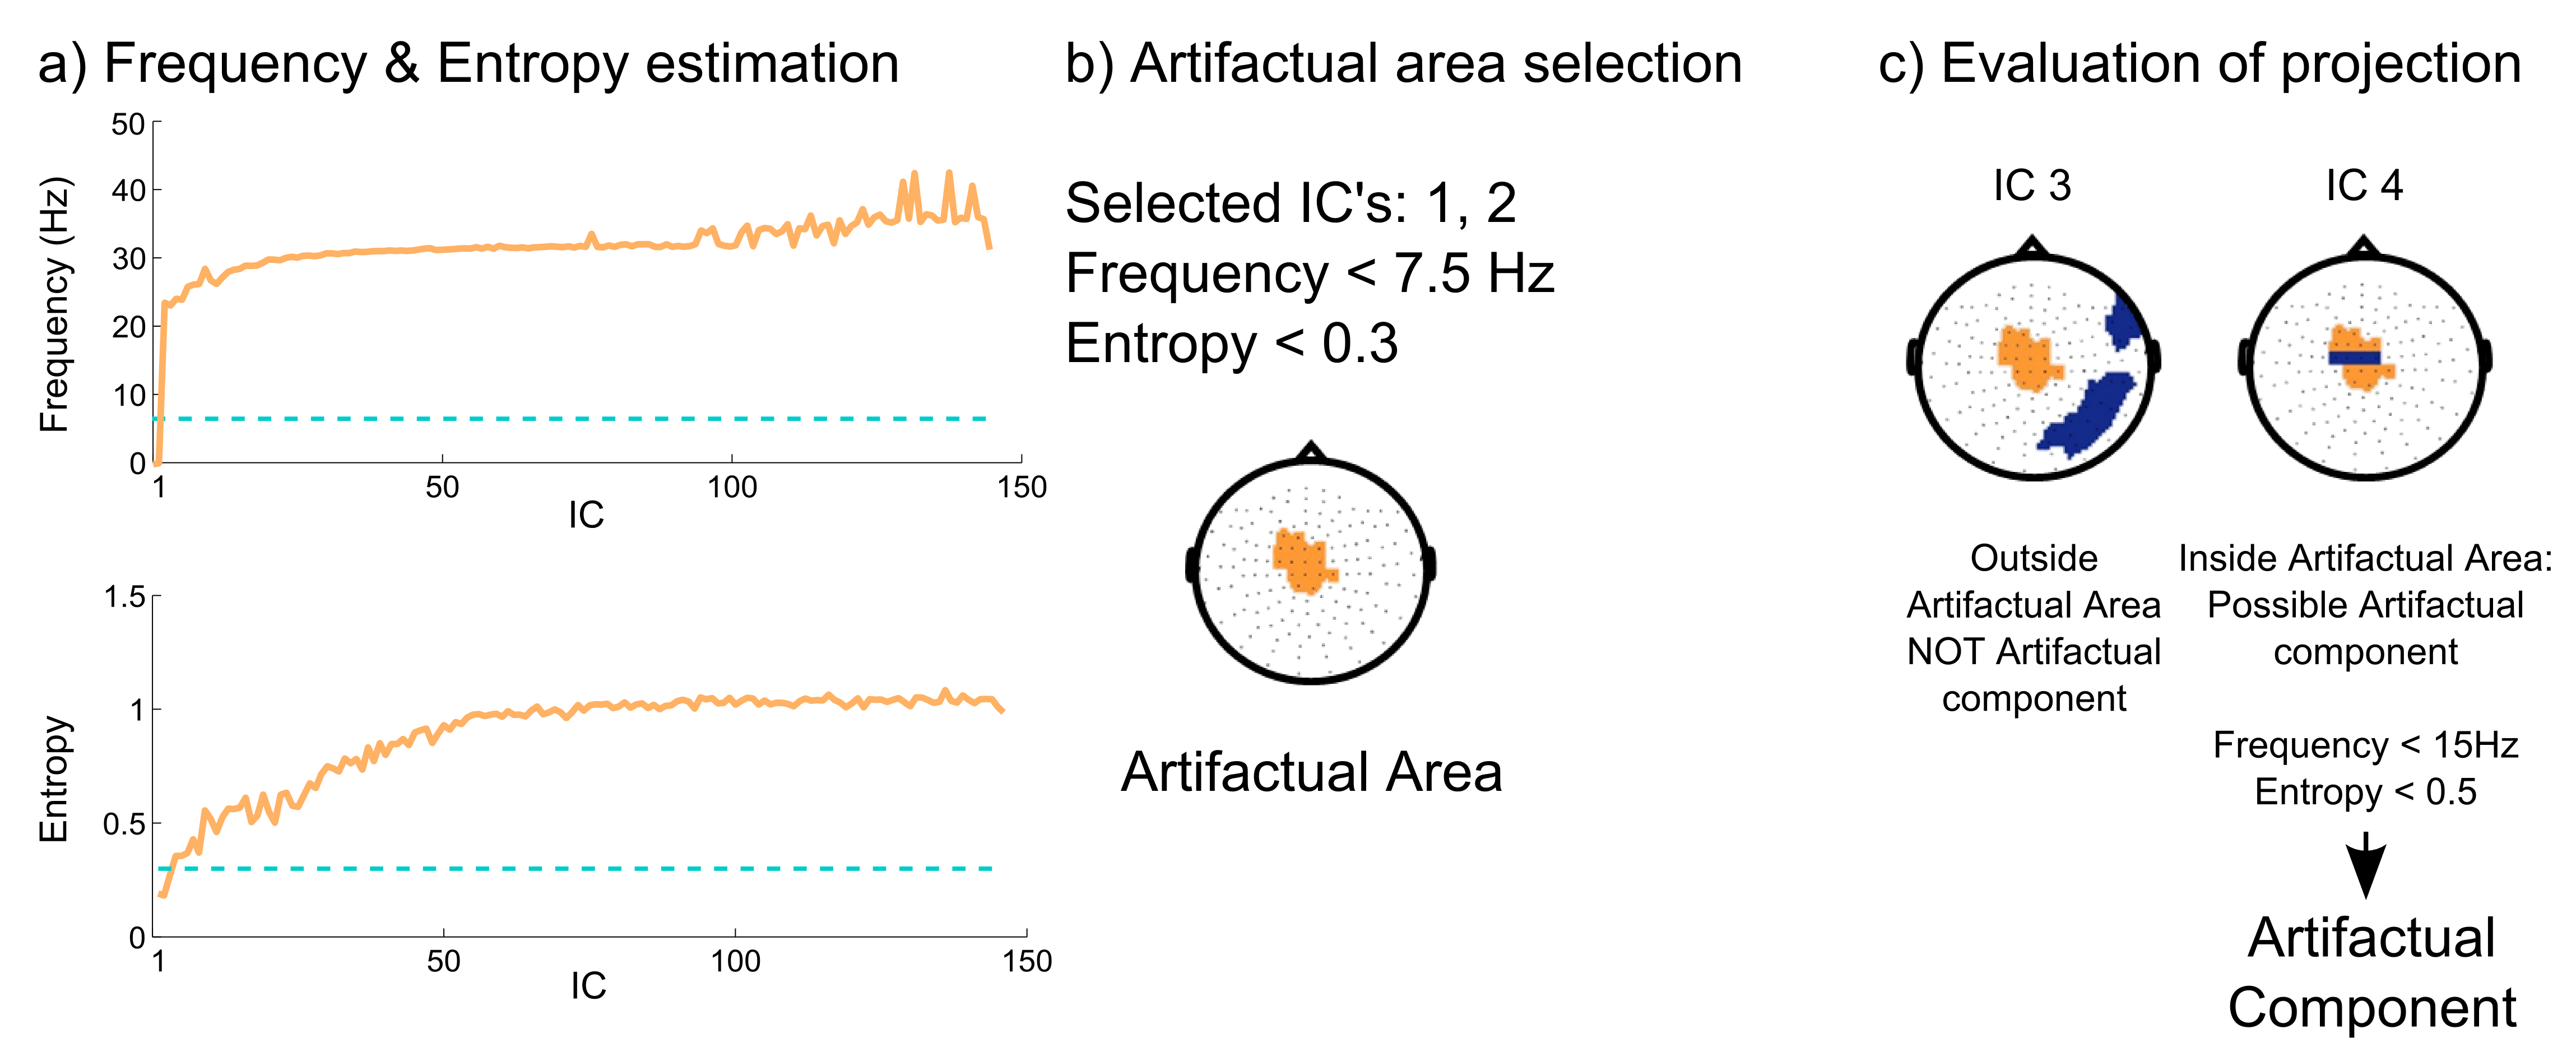
\includegraphics[width=1\textwidth]{Images/fig1-2.png}
\caption{Automatic artifact-related component selection: (a) frequency and entropy estimation (for all extracted ICs) and thresholds (blue dashed lines). (b) Artifactual area selected by the union of the regions of interest of the selected ICs. (c) As an example, evaluation of the projection of ICs 3 and 4 is shown. Regions of interest are indicated with dark blue shading. IC 3 is outside the artifactual area and therefore would not be selected by the automatic algorithm, whereas IC 4 would, as its region of interest is inside the artifactual area and the weak criteria concerning frequency and entropy are met.}
\label{fig:1-2}
\end{figure}      

The procedure carried out in order to select the artifactual components was based on two steps: the selection of the artifactual region and a comparison of this region with the projection of each IC.

The purpose of the first step was to locate the artifactual area that, due to the particular origin of metallic artifacts, could be located anywhere on the scalp. In this first step, those components which simultaneously met the two above-mentioned criteria were selected as artifactual components (figure \ref{fig:1-2}(b)) and used to identify the area of the scalp where the artifact was located. A strong version of the criteria was applied, and only ICs with 90\% of the energy in the slowest frequency bands delta and theta (up to 7.5 Hz) and high regularity (sample entropy lower than 0.3, obtained with an embedding dimension of 3 and a search radius of 0.1 times the standard deviation of the signal) were selected.

A region of interest was defined for each selected component, taking into account the BSS weights normalized with respect to the maximum for each channel and discarding the lowest quartile. The final artifactual region was defined as the union of the regions of each component. The purpose of this selection was to define a region where the artifact projected and to prevent artifactual regions being focused on only a few high-energy channels.

The second step involved the comparison between the artifactual region and the region of interest of every IC (figure \ref{fig:1-2}(c)). When this region of interest was included in the artifactual region and an IC fulfilled a weak version of the aforementioned criteria (90\% of energy below 15 Hz, sample entropy lower than 0.5), then the IC under evaluation was marked as an artifactual component. This second step was performed in order to ensure the selection of artifactual components that displayed characteristics highly related to metallic interference and were focused on the defined artifactual region. To achieve an effective removal of metallic interference, all marked ICs had to be removed, and the resulting artifact-free signal was obtained as the product of the remaining components by the weight matrix obtained by the algorithm.

\subsection{Performance assessment}

In order to assess the performance of the metallic artifact removal methodology, several error measurements based on time and frequency domain were calculated for each channel and each simulated recording.

\begin{enumerate} [(i)]
\item The normalized mean squared error (nMSE),
  \begin{equation}
	NMSE_n = 100 \cdot \frac{\sum_{i}^{N} (x_{n}(i)-y_{n}(i))^2}{\sum_{i}^N y_{n}(i)^2}
  \end{equation}
  
\item The variation of absolute power in the delta band (0.5 to 4 Hz) was obtained to study the error in the band most affected by metallic artifacts.
 \begin{equation}
	\bigtriangleup \delta  = 100 \cdot \frac{{\delta}_x -{\delta}_y}{{\delta}_y}
  \end{equation}

where ${\delta}_x$ and ${\delta}_y$ represent the power of the $\delta$ band of the filtered MEG channel under evaluation and of the original clean signal respectively.


\item The variation of absolute power in the alpha band (7.5 to 13 Hz) was also calculated in order to observe the error made in a band where metallic artifacts should have little influence, and therefore errors should be lower.
  
  \begin{equation}
	\bigtriangleup \alpha  = 100 \cdot \frac{{\alpha}_x -{\alpha}_y}{{\alpha}_y}
  \end{equation}
\end{enumerate}

where ${\alpha}_x$ and ${\alpha}_y$ represent the power in the $\alpha$ band of the signal under evaluation and of the original clean signal respectively.

\section{Results}

\subsection{Simulated data}

Ten simulated datasets were generated following the steps explained in figure \ref{fig:1-1}. The number of channels containing visible metallic interference selected by the experts was 6.6 $\pm$ 4.4, and, in general, artifacts contaminated channels with varying amplitudes. While in some subjects the high amplitude of the artifacts affected many channels, there were other cases where high amplitudes focused on a reduced number of channels. In spite of the dispersion shown by the location of the artifact, their associated signals showed low frequency and regular pattern characteristics, modulated by cardiac and respiratory rates.

Once the different waveforms (patterns) were obtained, and after proper filtering and correlation procedures explained in the previous sections, propagation to the whole head was performed by means of linear regression. Figure \ref{fig:1-3} shows the propagation coefficients normalized with respect to the maximum obtained after regression. It is noticeable that metallic artifacts affected different areas of the scalp depending on the subject, and while in some cases artifacts were focused at specific regions, in others they appeared more dispersed and covered a larger area of the head.

\begin{figure}[ht]
\centering
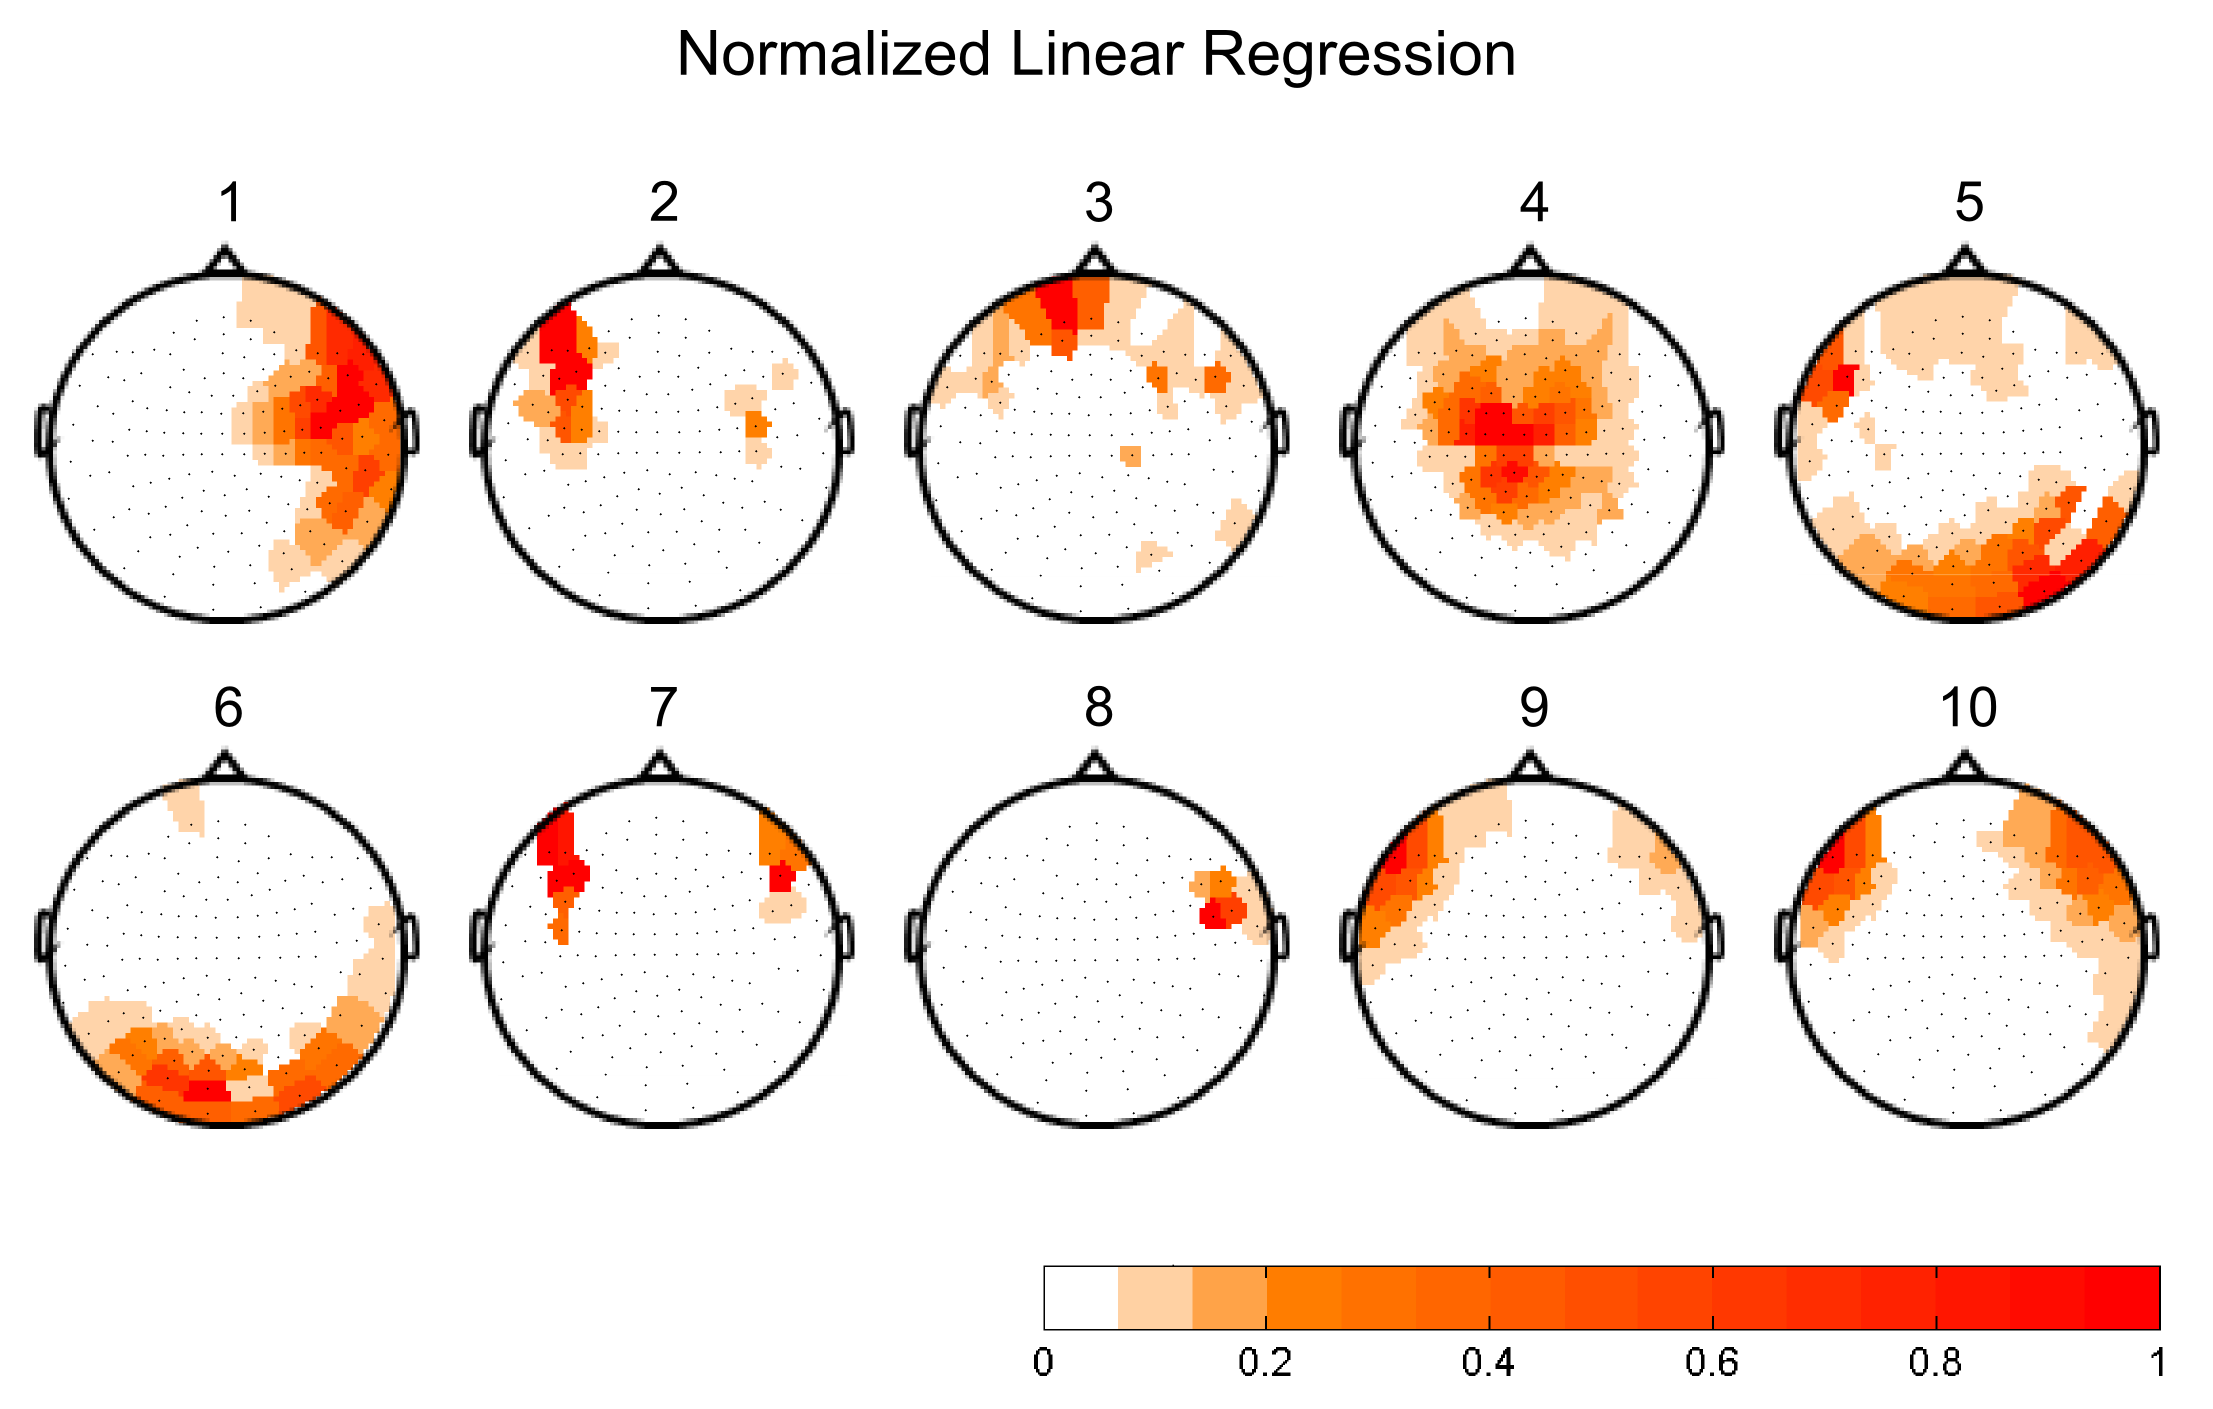
\includegraphics[width=0.9\textwidth]{Images/fig1-3.png}
\caption{Sum of the linear regression coefficients normalized with respect to its maximum for all of the selected artifactual patterns for the 10 simulated MEG sets. Coefficients were obtained for the whole head after morphology selection and linear regression of each channel with the selected morphologies. Note that metallic artifacts behave differently depending on their nature and therefore they can appear in different areas of the head for each simulated MEG set.}
\label{fig:1-3}
\end{figure}      

\subsection{Blind source separation and automatic detection}

Separation of ICs was performed with AMUSE, INFOMAX and FastICA for the ten simulated subjects. AMUSE and INFOMAX algorithms successfully extracted ICs from the mixed signals in which artifact-related source components where visually identifiable. Subgaussianity of the data, especially related to metallic artifacts, caused a non-effective decomposition in the case of the FastICA algorithm, which could not separate ICs related to brain signals from metallic artifacts even after using the stabilization parameters to ensure convergence.

The automatic detection procedure was applied to the obtained ICs to detect which components were associated with the metallic interference and therefore were to be discarded to obtain a successful removal of metallic artifacts.

Figure \ref{fig:1-4}(a) shows, as an example, an artifact-free subject signal; and figure \ref{fig:1-4}(b) shows the simulated signals obtained after the addition of artifactual waveforms to the same subject. Figure \ref{fig:1-5} shows the results, in time domain, of the artifact reduction process on simulated signals shown in figure \ref{fig:1-4}. Figures \ref{fig:1-5}(a), (b) and (c) show the extracted ICs for AMUSE, INFOMAX and FastICA respectively, with the selected ICs displayed in a different color. The resulting signals obtained after reconstruction without considering the ICs associated with metallic interference are shown in figures \ref{fig:1-5}(d), (e) and (f). It is noticeable that the automatic algorithm procedure was not able to identify any metallic-related ICs in the FastICA decomposition, and this led to a full reconstruction of the signal with the original metallic interference. Visual inspection of the extracted components and the reconstructed signals indicated that INFOMAX was not completely successful in separating brain-related activity from artifactual waveforms, but AMUSE was indeed able to separate metallic interference from MEG activity. INFOMAX provided components related to artifactual activity mixed with cerebral waveforms and the effects of such a decomposition were remarkable after signal reconstruction (figure \ref{fig:1-5}(e)), especially when compared to AMUSE (figure \ref{fig:1-5}(d)), which showed much more similar signals compared to the clean set (figure \ref{fig:1-4}(a)).

\begin{figure}[ht]
\centering
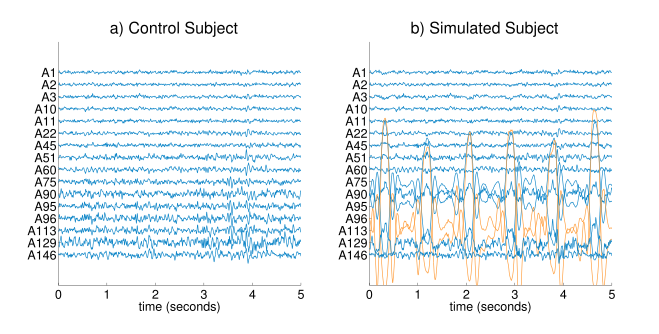
\includegraphics[width=1\textwidth]{Images/fig1-4.png}
\caption{MEG channels (16 distributed evenly on the scalp) for: (a) control subject, that is, clean recording, free of metallic artifacts; (b) simulated subject. Orange traces indicate channels originally selected as artifacts by the experts.}
\label{fig:1-4}
\end{figure}   

\begin{figure}[ht!]
\centering
\hspace*{-0.7cm}
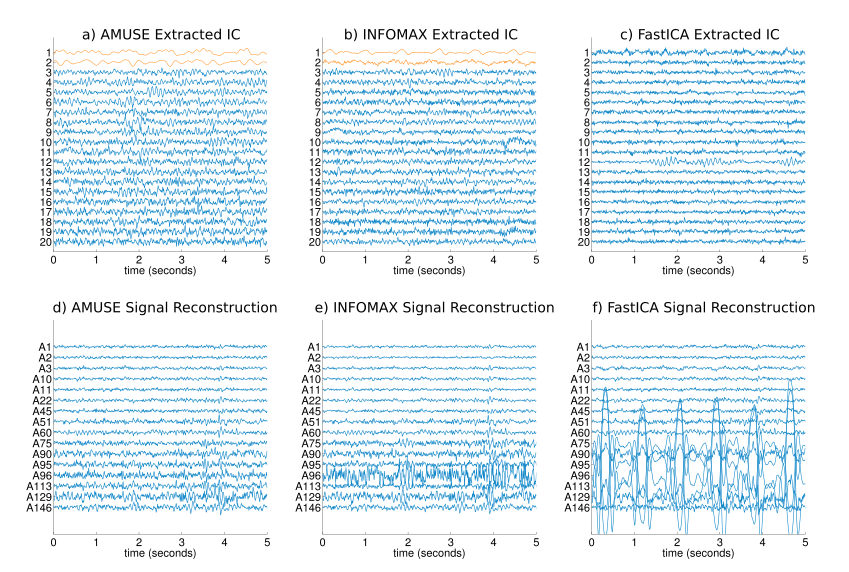
\includegraphics[width=1.1\textwidth]{Images/fig1-5.png}
\caption{ Artifact-reduction for a simulated subject: (a), (b) and (c) show the first 20 extracted ICs corresponding to AMUSE, INFOMAX and FastICA algorithms, respectively. Note that the first 2 ICs (orange traces) obtained by AMUSE and INFOMAX were automatically selected and removed to perform signal reconstruction, whose results are shown in (d) and (e), respectively. FastICA was not able to extract useful artifact-related components and the reconstruction shown in (f) does not remove any amount of artifact (and, consequently, the reconstructed signals equal those of figure \ref{fig:1-4}(b)).}
\label{fig:1-5}
\end{figure}   

\subsection{Performance assessment}

Figure \ref{fig:1-6} shows the percentage error in several subjects as an example, represented as whole-head topographic maps. These errors were calculated for three conditions: simulated signals without correction, to observe the amount of artifact introduced; and after applying AMUSE- and INFOMAX-based artifact filtering. Metallic contamination was mainly present in the area of high-energy artifacts, while the distortion of the remaining channels was considerably lower. For this reason the amount of error observed for the uncorrected case always showed a maximum error value in the artifactual region. As expected, errors in the delta frequency band after filtering were higher than in the alpha band because of the characteristics of metallic contamination, and INFOMAX showed higher errors than AMUSE.

\begin{figure}[ht!]
\centering
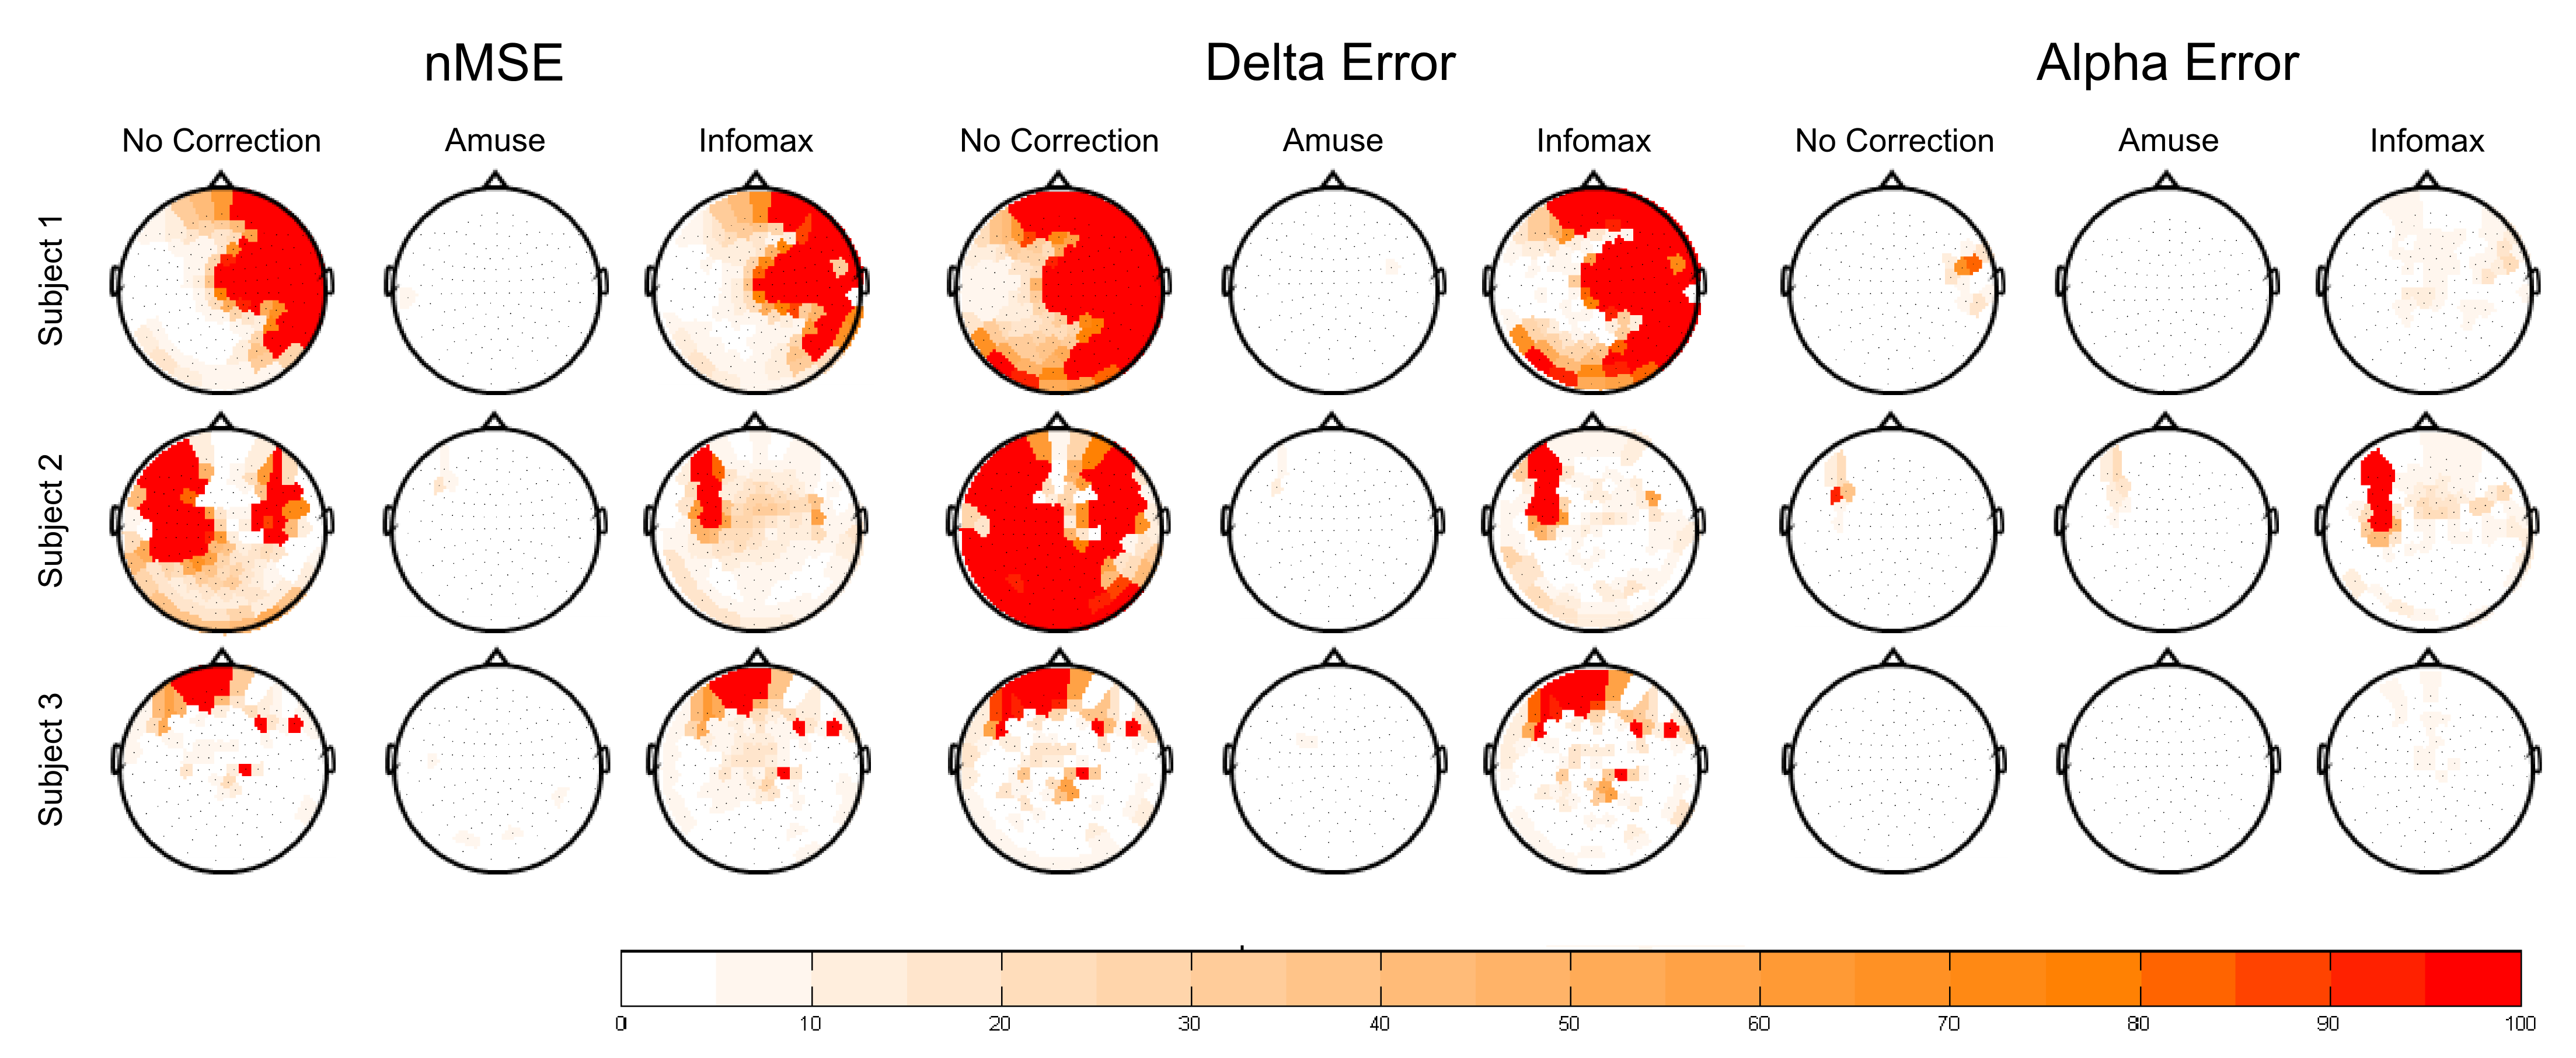
\includegraphics[width=1\textwidth]{Images/fig1-6.png}
\caption{Error percentage for normalized MSE, delta power and alpha power, shown for three different simulated subjects as examples. Errors are shown for non-corrected, AMUSE-corrected and INFOMAX-corrected signals. Due to the frequency content of metallic artifacts, errors are expected to be lower in the alpha band and higher in the delta band, focusing especially on the areas where the artifact is located. Note that AMUSE-based reconstruction shows the lowest errors for the three measures.}
\label{fig:1-6}
\end{figure}  

As explained in the previous sections, metallic contamination masked the cerebral activity of some channels in real cases. This situation was reproduced in the simulated MEG subjects and, in fact, the energy introduced by metallic artifacts in MEG activity was huge in many cases (see values and average in table \ref{tb:1-1}). After applying INFOMAX-based correction, this error was reduced but still high, whereas after AMUSE-based filtering this error was lower than 1\%.


\begin{table}[ht!]
\centering
\caption{Error percentage for nMSE, delta power and alpha power (average of all channels) for non-corrected signals, AMUSE-corrected signals and INFOMAX-corrected signals.}
\small
\vspace{3mm}
\hspace*{-0.35cm}
\label{tb:1-1}
\begin{tabular}{rrrrrrrrrr}
\multicolumn{1}{l}{} & \multicolumn{3}{c}{nMSE}                                                                           & \multicolumn{3}{c}{Delta error (\%)}                                                               & \multicolumn{3}{l}{Alpha Error (\%)}                                                                   \\ \hline
\multicolumn{1}{l}{} & \multicolumn{1}{l}{}                                 & \multicolumn{1}{l}{} & \multicolumn{1}{l}{} & \multicolumn{1}{l}{}                                 & \multicolumn{1}{l}{} & \multicolumn{1}{l}{} & \multicolumn{1}{l}{}                                     & \multicolumn{1}{l}{} & \multicolumn{1}{l}{} \\ 
Subj.                & \begin{tabular}[c]{@{}r@{}}Non-\\ corrected \end{tabular} & Amuse                & Infomax              & \begin{tabular}[c]{@{}r@{}}Non-\\ corrected \end{tabular} & Amuse                & Infomax              & \begin{tabular}[c]{@{}r@{}}Non-\\ corrected\end{tabular} & Amuse                & Infomax              \\ \hline
\multicolumn{1}{l}{} & \multicolumn{1}{l}{}                                 & \multicolumn{1}{l}{} & \multicolumn{1}{l}{} & \multicolumn{1}{l}{}                                 & \multicolumn{1}{l}{} & \multicolumn{1}{l}{} & \multicolumn{1}{l}{}                                     & \multicolumn{1}{l}{} & \multicolumn{1}{l}{} \\
1                    & 521.70                                               & 0.12                 & 414.10               & 2464.23                                              & 0.52                 & 2226.07              & 2.12                                                     & 0.31                 & 3.99                 \\
2                    & 7811.33                                              & 0.33                 & 173.02               & 44500.04                                             & 0.42                 & 214.46               & 1.30                                                     & 0.88                 & 121.7                \\
3                    & 43.94                                                & 0.02                 & 48.02                & 84.01                                                & 0.15                 & 83.93                & 0.02                                                     & 0.07                 & 2.15                 \\
4                    & 20926.17                                             & 1.51                 & 3622.56              & 64421.30                                             & 2.50                 & 12293.77             & 0.97                                                     & 2.52                 & 475.44               \\
5                    & 219.99                                               & 0.02                 & 19.68                & 1568.38                                              & 0.13                 & 131.80               & 0.01                                                     & 0.06                 & 2.06                 \\
6                    & 3754.65                                              & 0.21                 & 50.55                & 14169.41                                             & 0.48                 & 66.97                & 32.76                                                    & 0.62                 & 42.49                \\
7                    & 9061.74                                              & 0.57                 & 3417.17              & 59869.96                                             & 0.80                 & 9964.57              & 0.01                                                     & 0.44                 & 1665.48              \\
8                    & 8379.42                                              & 0.19                 & 135.58               & 43106.98                                             & 0.22                 & 174.84               & 0.01                                                     & 0.12                 & 114.64               \\
9                    & 3795.21                                              & 0.13                 & 45.05                & 14018.33                                             & 0.64                 & 39.15                & 121.08                                                   & 0.52                 & 38.35                \\
10                   & 3764.70                                              & 0.59                 & 205.70               & 14720.35                                             & 1.33                 & 308.99               & 148.16                                                   & 2.01                 & 102.39               \\
\multicolumn{1}{l}{} & \multicolumn{1}{l}{}                                 & \multicolumn{1}{l}{} & \multicolumn{1}{l}{} & \multicolumn{1}{l}{}                                 & \multicolumn{1}{l}{} & \multicolumn{1}{l}{} & \multicolumn{1}{l}{}                                     & \multicolumn{1}{l}{} & \multicolumn{1}{l}{} \\
\textbf{Mean}        & \textbf{5827.89}                                     & \textbf{0.37}        & \textbf{813.14}      & \textbf{25892.30}                                    & \textbf{0.72}        & \textbf{2550.45}     & \textbf{30.64}                                           & \textbf{0.75}        & \textbf{256.87}     
\end{tabular}
\end{table}

The variability in amplitude and energy of metallic artifacts caused the amount of error introduced to be very inhomogeneous. As can be observed in figure \ref{fig:1-6}, INFOMAX was not an appropriate method to remove the interference because of the large amount of error obtained: the error provided in the alpha band, sometimes higher than without correction, suggested that INFOMAX ICs associated with artifacts were a mixture of metallic and cerebral signals, and possibly some brain-related activity was being deleted. On the contrary, AMUSE always provided low alpha power errors, below 3\%.

\subsection{Real data}

Once the effectiveness of the automatic BSS-based procedure has been measured using simulated signals, assessment of its performance with real MEG data is pertinent. Real spontaneous MEG signals with eyes closed corresponding to the 10 subjects with ferromagnetic implants described in the 'Materials and Methods' section were used for this purpose. One way to demonstrate the filtering performance is to show that alpha-band oscillations with eyes closed can be better detected after artifact removal.

Figure \ref{fig:1-7}(a) shows as an example a five-second epoch corresponding to a subject with a metallic subdural grid affecting the posterior region of the scalp where a high interference is clearly noticeable. The AMUSE algorithm, which has been shown to be the most effective and efficient technique in the simulated database, was used for the BSS decomposition. After applying the filtering procedure (see figure {fig:1-7}(b)), alpha waves could be easily recognized by visual inspection. Moreover, topographic maps of the average alpha power of the 10 subjects with metallic implants before and after applying the automatic procedure are shown in figure {fig:1-8}. Although metallic artifacts mainly affected the delta and theta bands, the alpha-band is also significantly affected, as shown in figure {fig:1-8}(a) where alpha power is scattered over the scalp due to metallic interference. Once the BSS-based artifact reduction procedure was applied, the map shows a physiologically more plausible distribution of alpha power mainly focused on the posterior region, as expected.

\begin{figure}[ht]
\centering
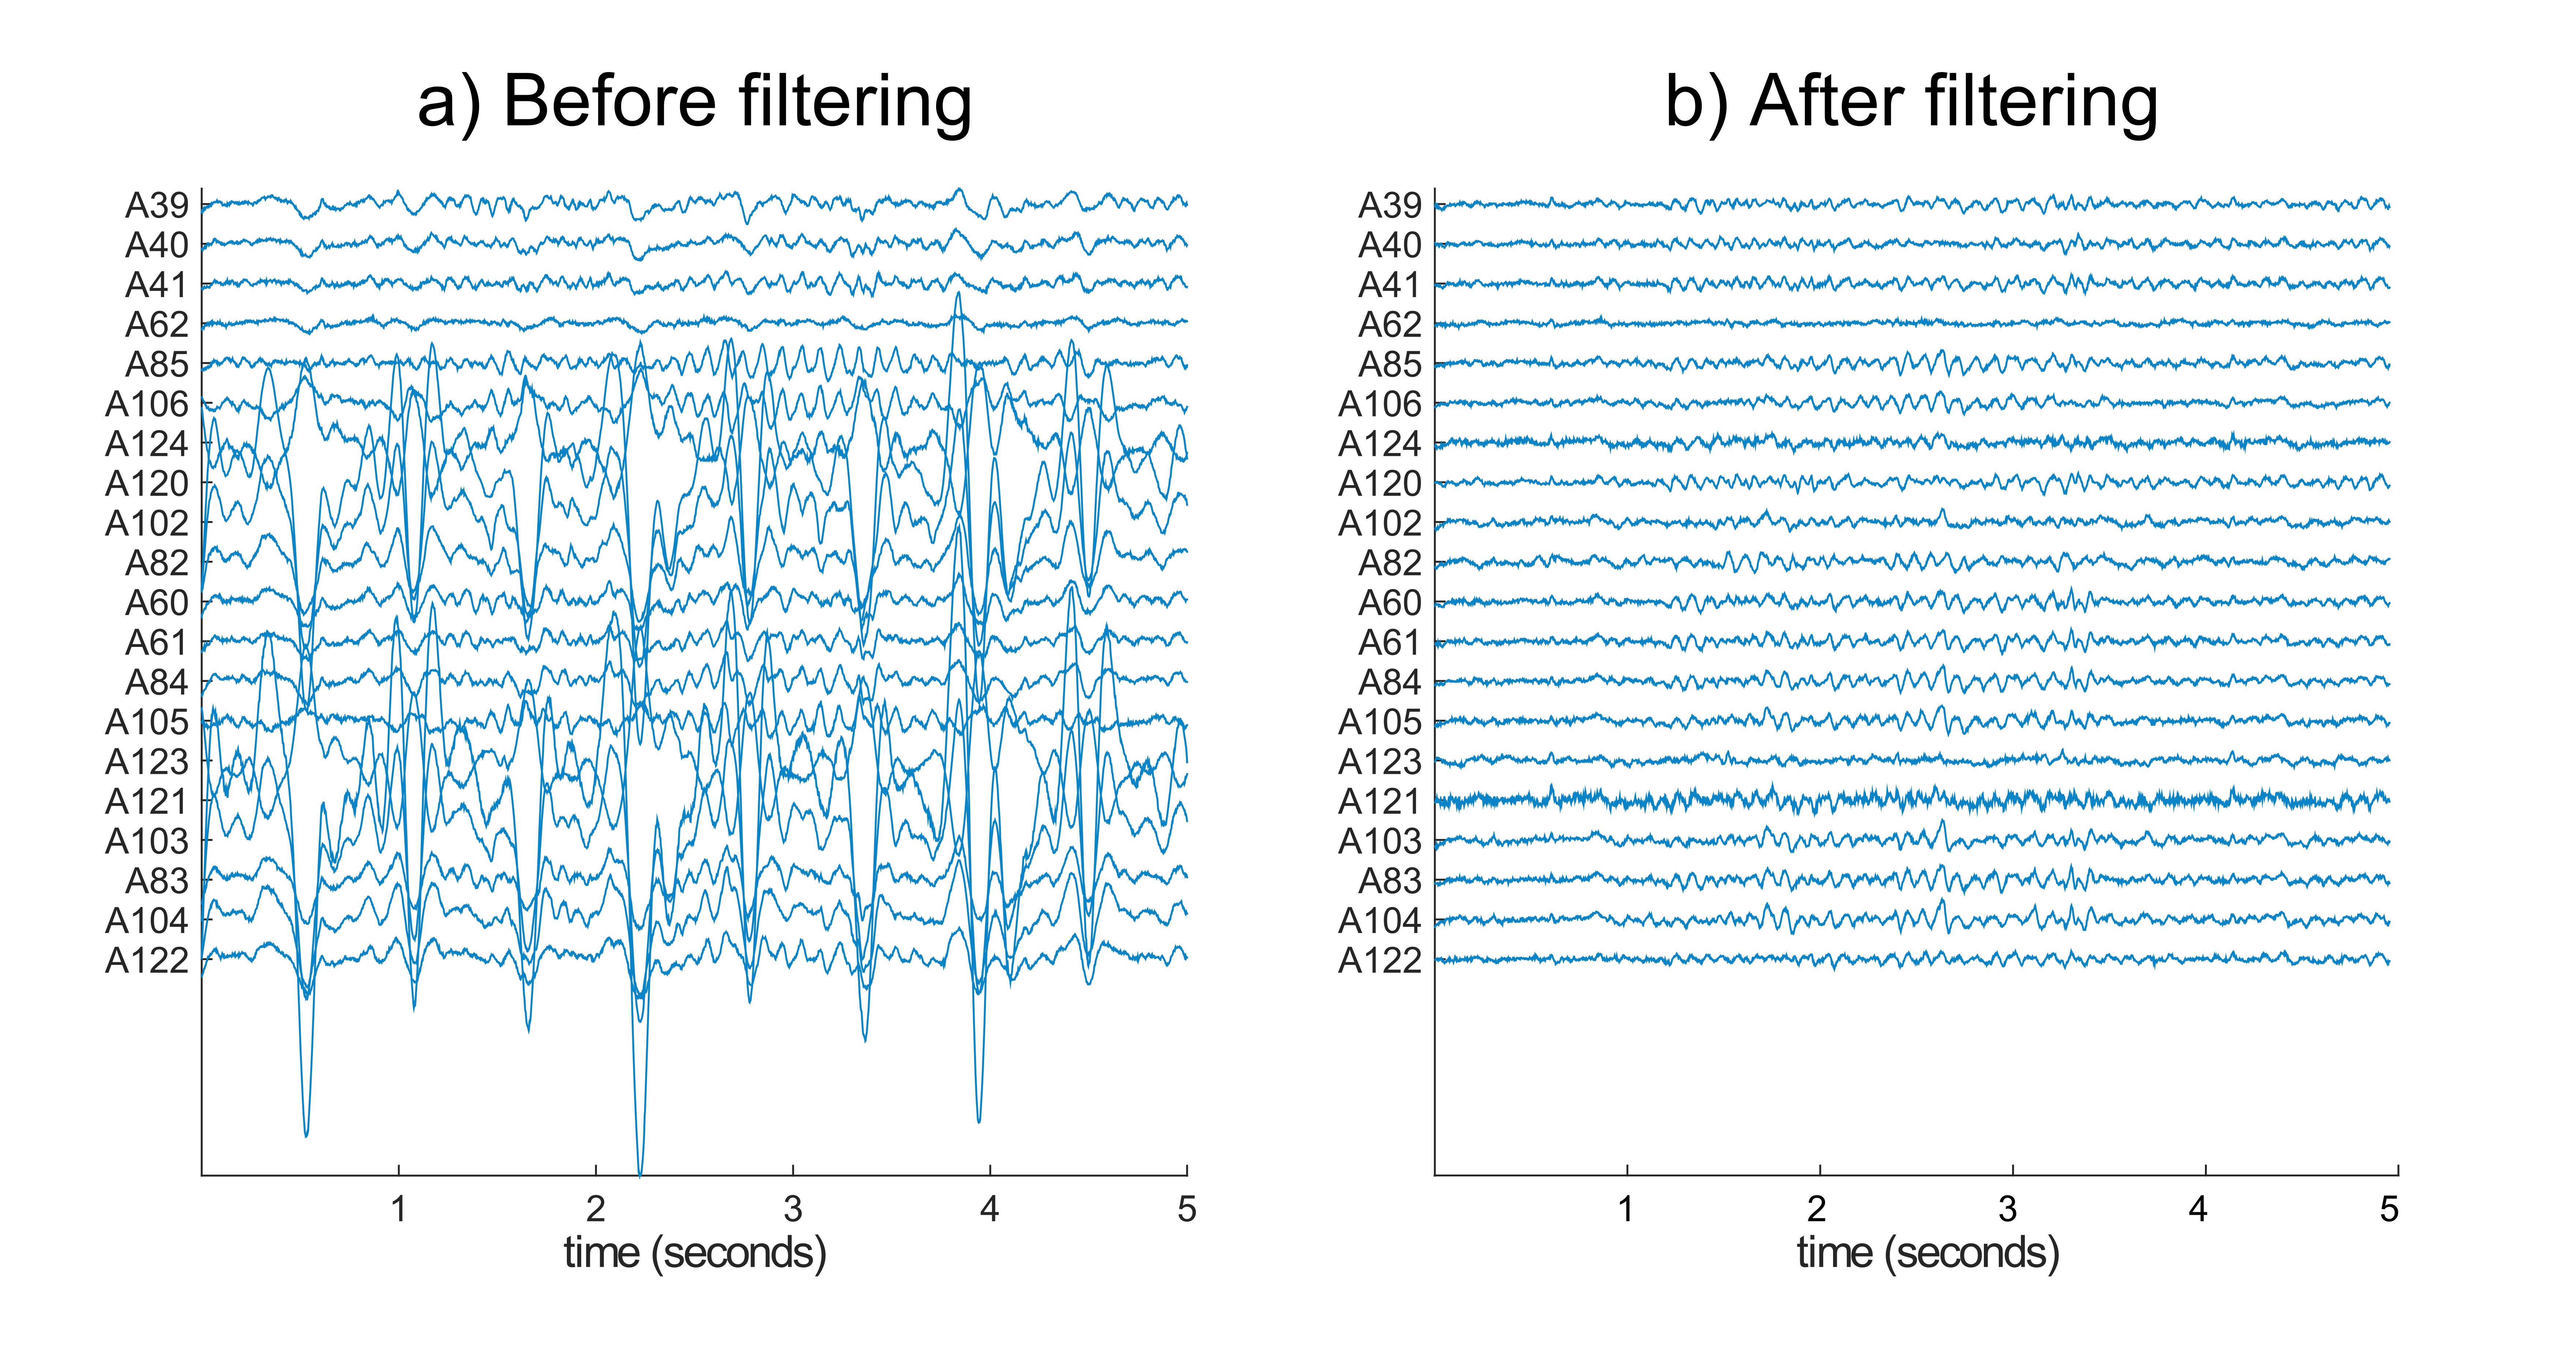
\includegraphics[width=1\textwidth]{Images/fig1-7.png}
\caption{(a) Five-second epoch of raw MEG signals containing prominent metallic interference. Posterior channels are shown as an example. (b) Corrected MEG signals obtained after applying automatic AMUSE-based metallic removal procedure.}
\label{fig:1-7}
\end{figure}  

\begin{figure}[ht]
\centering
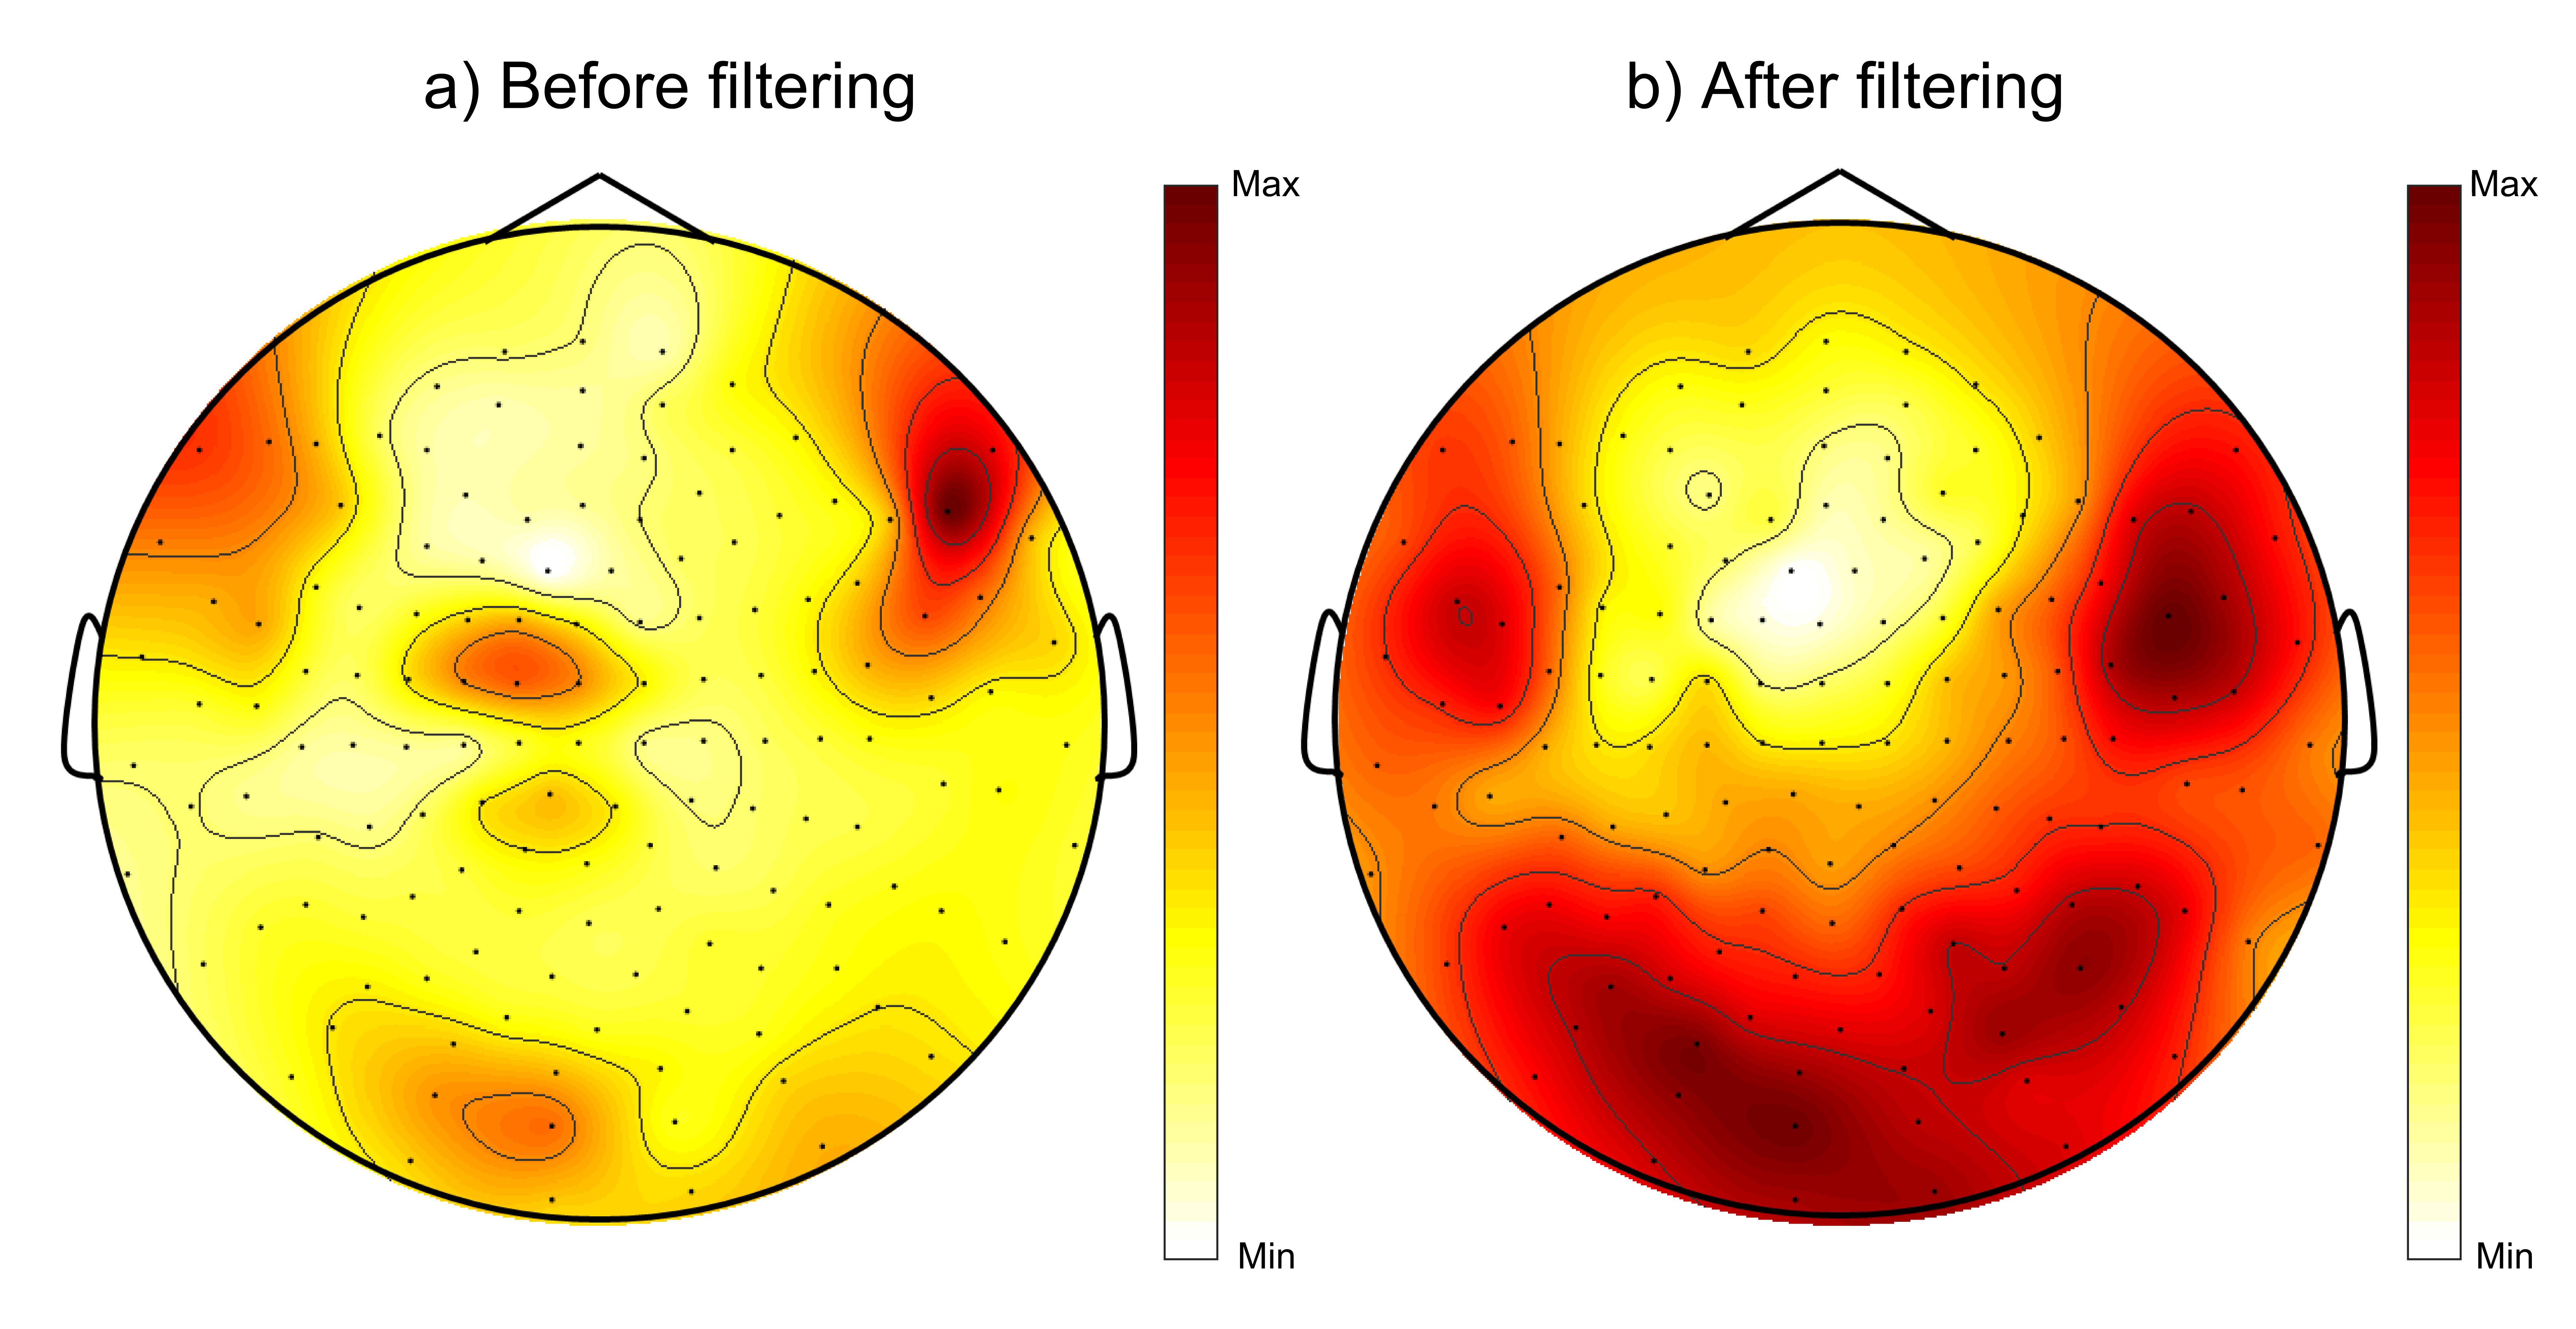
\includegraphics[width=1\textwidth]{Images/fig1-8.png}
\caption{(a) Topographic distribution of the average alpha power of the 10 artifactual subjects. (b) Average of alpha power obtained after applying automatic AMUSE-based metallic removal procedure.}
\label{fig:1-8}
\end{figure} 

\section{Discussion}

Metallic artifacts in MEG recordings are an important issue in the diagnosis of neurobiological events because they can hugely distort MEG signals and render many single-channel signals unusable. This leads to an unavoidable loss of information regarding the activity of the brain, or even worse, to a rejection of the MEG technique as a mean to obtain reliable cerebral signals of those patients who have metallic elements that could generate such interferences.

Signal space separation (SSS) \citep{Taulu2004} and temporal SSS (tSSS) \citep{Taulu2006} are also methods for MEG filtering. Applying SSS or tSSS is highly advised for Elekta-Neuromag systems \citep{GonzalezMoreno2014} and their algorithms are provided by a software registered and available only on this equipment. On the other hand, the filtering approach presented in this paper is based on BSS standard libraries which are freely available and could be used with signals from different MEG systems such as CTF/VSM, 4D Neuroimaging, Elekta and Yokogawa.

The tSSS algorithm was applied efficiently to remove MEG artifacts in several studies \citep{GonzalezMoreno2014,Nenonen2012,Taulu2009} and in particular, in the case of metallic interferences: \citep{Hillebrand2013,Cheyne2007,Taulu2006}. These studies showed the improvement of dipole fitting procedures when tSSS is applied instead of SSS but they did not evaluate the noise reduction of metallic interference or measure it quantitatively. Furthermore, there are no comparative studies of this technique with other artifact reduction algorithms such as BSS or epoch rejection.

In \citep{GonzalezMoreno2014} an interesting SNR analysis was carried out when SSS and tSSS were first applied followed by the BSS or epoch-rejection procedure. This study concluded that SNR increased by 100\% after applying SSS or tSSS techniques. Moreover, the SNR improved an additional 33–36\% when BSS methods were subsequently applied. The latter suggests that not all noise was successfully removed by the tSSS method and BSS algorithms could remove interferences that remained after applying tSSS techniques. In addition, these studies also concluded that one of the main drawbacks of BSS-based noise-reduction techniques is the need for manual selection of noisy or artifactual components, which is done visually. However, our study describes an automatic approach to detect artifactual components.

As the location and intensity of metallic artifacts usually varies among different subjects, it is not possible to make feasible \textit{a priori} assumptions on these characteristics to adjust an automatic detection algorithm. In this work, a new BSS-based automatic procedure using freely available standard libraries was presented to identify components related to metallic activity, whose performance was tested using simulated MEG signals, which are essential to objectively quantify the effectiveness of the method while reproducing standard clinical situations as faithfully as possible.

One of the main questions arising when working with BSS is the estimation of the number of independent components (ICs) to be extracted. At most, it is possible to extract as many ICs as there are channels that the record is composed of, but when this number is high it is usually advisable to reduce it and usually a lower number of ICs is obtained. The search for the optimal number allows one to avoid over- and under-fitting phenomena \citep{Li2007},  and is often achieved by selecting the ICs that can explain a high percentage of the variance of the signals. Due to the high amount of energy accounted for by metallic artifacts, the reduction of the number of ICs was not appropriate when dealing with this kind of interference. The energy of the artifacts was much greater than that of cerebral signals (around four orders of magnitude in some cases) and consequently the number of ICs corresponding to very high percentages of the total variance resulted in being very low. Thus, it was not possible to achieve a successful separation between cerebral activity and metallic interferences. For this reason, all BSS algorithms were forced to extract as many components as available channels.

One Second-Order Statistics (SOS) and two Higher-Order Statistics (HOS) techniques were tested. The SOS-based algorithm, AMUSE, showed considerably lower errors and therefore a valid decomposition. In the case of HOS, two algorithms were tested, INFOMAX and FastICA. While the first one was successful in separating ICs related to brain activity from those of metallic interference, the second did not manage to generate a valid decomposition. FastICA is an algorithm that uses the kurtosis to evaluate the gaussianity in order to separate independent components. This algorithm is very effective in dealing with supergaussian sources such as cardiac and ocular interferences (kurtosis higher than 3), but its principal drawback is poor convergence when working with gaussian and subgaussian signals, which is the case for metallic interferences that, in general, present a kurtosis value close to 3. Even after ensuring convergence by means of the stabilizer provided by \citep{Hyvarinen1999}, the decomposition was not effective and no metallic-related components could be identified.

On the other hand, the extended version of INFOMAX was able to work with subgaussian signals, and effective convergence and IC separation were achieved. However, the algorithm was not able to separate metallic components as accurately as AMUSE, and part of the cerebral signals remained, mixed with metallic components. That is the main reason why some of the error measures increased significantly when INFOMAX was applied.

After source decomposition, a simple two-step procedure for metallic-related component identification was applied. This simple scheme, based on two criteria which exploited the basic characteristics of metallic artifacts (low frequency and regularity), allowed the delimitation of an artifactual region. Once this region was obtained, all possible ICs that exhibited artifactual behavior were identified and removed from the reconstruction matrix.

This artifact-filtering methodology was tested on 10 sets of simulated MEG signals consisting of clean recordings to which metallic artifacts were added. The extraction of these artifacts from real signals was performed taking into account the different morphologies and varying propagation of this contamination by means of filtering, correlation and estimation of propagation coefficients by linear regression.

Results showed that the two-step automatic detection methodology was able to detect ICs related to metallic interference especially when they were extracted through the AMUSE algorithm. Normalized MSE error showed and average value of 0.37\% (see table \ref{tb:1-1}). Errors in delta power were lower than 1\% in average, showing a great performance in the most affected spectral band.

It is notable that these error measures presented very low values when compared to non-corrected sets of signals. However, there were some cases in which alpha power showed a slightly higher error (worst case subject 4, 1.55\% in excess) but this amount can be considered negligible with respect to the general improvement achieved.

Moreover, the performance of the automatic BSS reduction method was assessed in real MEG signals. Results showed that even high-amplitude metallic interference was properly removed from the MEG data. A study based on the alpha activity confirmed that the BSS-based procedure was able to reduce the metallic artifacts and show a more plausible topographic distribution of alpha-band signal after filtering.

Therefore, after applying the fully automated BSS procedure in simulated and real artifactual MEG data, it can be concluded that AMUSE is the most suitable technique to be used along with the two-step algorithm presented in this study for effectively removing metallic interference from MEG signals.

\section{Acknowledgments}

CIBER-BBN is an initiative of the Instituto de Salud Carlos III, Spain. This work has been partially supported by the Ministry of Economy and Competitiveness (MINECO), Spain, under contracts DPI2011-22680 and DPI2014-59049-R and the Ministry of Education, Culture and Sports (MECO) FPU12/05631.